%%%%%%%%%%%%%%%%%%%%%%%%%%%%%%%%%%%%%%
% TRB Poster 2015
% Created by Subasish Das
% January 2015
%%%%%%%%%%%%%%%%%%%%%%%%%%%%%%%%%%%%%%

\documentclass[final]{beamer}
\usepackage[scale=1.24]{beamerposter}
\usepackage{graphicx}			% allows us to import images

%-----------------------------------------------------------
% Custom commands that I use frequently
%-----------------------------------------------------------

\newcommand{\bb}[1]{\mathbb{#1}}
\newcommand{\cl}[1]{\mathcal{#1}}
\newcommand{\fA}{\mathfrak{A}}
\newcommand{\fB}{\mathfrak{B}}
\newcommand{\Tr}{{\rm Tr}}
\newtheorem{thm}{Theorem}

%-----------------------------------------------------------
% Define the column width and poster size
%-----------------------------------------------------------

\newlength{\sepwid}
\newlength{\onecolwid}
\newlength{\twocolwid}
\setlength{\paperwidth}{48in}
\setlength{\paperheight}{36in}
\setlength{\sepwid}{0.024\paperwidth}
\setlength{\onecolwid}{0.22\paperwidth}
\setlength{\twocolwid}{0.464\paperwidth}
\setlength{\topmargin}{-0.5in}
\usetheme{confposter}
\usepackage{exscale}


\usecaptiontemplate{
\small
\structure{\insertcaptionname~\insertcaptionnumber:}
\insertcaption}

%-----------------------------------------------------------
% Define colours (see beamerthemeconfposter.sty to change these colour definitions)
%-----------------------------------------------------------

\setbeamercolor{block title}{fg=Mahogany,bg=white}
\setbeamercolor{block body}{fg=Black,bg=white}
\setbeamercolor{block alerted title}{fg=white,bg=Maroon!70}
\setbeamercolor{block alerted body}{fg=black,bg=ForestGreen!10}

%-----------------------------------------------------------
% Name and authors of poster/paper/research
%-----------------------------------------------------------

\title{A Comprehensive Study on Pavement Edge Line Implementation}
\author{Xiaoduan Sun, PhD \& PE, and, Subasish Das, PhD Candidate  \hspace{2in} ZhongJie "Doc" Zhang, PhD \& PE, Project Manager}
\institute{University of Louisiana \hspace{14in} Louisiana Transportation Research Center (LTRC) }

%-----------------------------------------------------------
% Start the poster itself
%-----------------------------------------------------------

\begin{document}
\begin{frame}[t]
  \begin{columns}[t]												% the [t] option aligns the column's content at the top
    \begin{column}{\sepwid}\end{column}			% empty spacer column
    \begin{column}{\onecolwid}
      \begin{alertblock}{Research Question}
        {\rmfamily{Will complying with the MUTCD 2000 regarding edge line implementation increase head on collisions on narrow rural roads in Louisiana?}}
      \end{alertblock}
      \vskip2ex
      \begin{figure}
              \begin{center}
                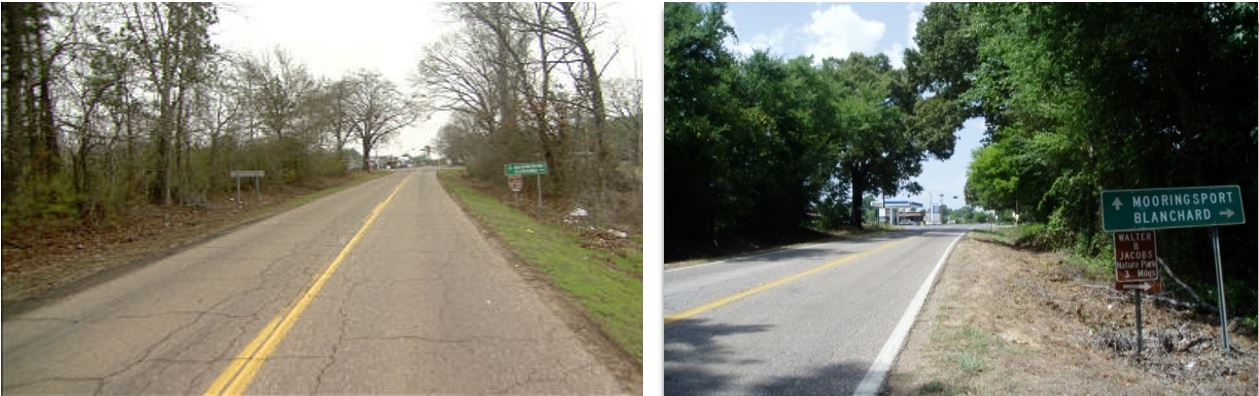
\includegraphics[width=10.5in, height= 3in]{abc.jpg}

              \end{center}
      \end{figure}
      \begin{block}{Background}
        {\rmfamily{Inexpensive crash countermeasure like pavement edge line helps to reduce roadway departures by providing a visual guidance that helps to confine vehicles within the travel lane. The MUTCD provides guidelines for the installation of edge lines. However, rural two-lane highways with narrow lane widths are not always required to have edge lines. While debating whether edge lines should be implemented on all rural two-lane highways to enhance roadway safety regardless of its lane width or Annual Average Daily Traffic (AADT), the state engineers had two concerns in particular. One of the concerns was that the presence of edge lines may influence drivers to operate closer to the centerline thus increasing the risks of head-on and sideswipe crashes. The other concern was additional cost.}}
      \end{block}
      \vskip2ex
      \begin{block}{Research Performed}
        {\rmfamily{\textbf{2005}\\
                \vspace{2mm}
                \textbf{\textit{Impact of Edge Lines on Safety of Rural Two-Lane Highways}}\\
                \vspace{2mm}
                \textbf{Goal:} To investigate if marking edge lines would have any negative effect on \textbf{drivers behavior} in decreasing road safety.\\
                \vspace{2mm}
                This study documented the results of past and present research and the current practices, investigated vehicle lateral positions under various roadway alignments and traffic conditions in one LaDOTD district, examined the potential tort liability, and developed a recommended guideline.
}}

      \end{block}
    \end{column}

    \begin{column}{\sepwid}\end{column}			% empty spacer column
    \begin{column}{\twocolwid}							% create a two-column-wide column and then we will split it up later
      \begin{columns}[t,totalwidth=\twocolwid]	% split up that two-column-wide column
        \begin{column}{\onecolwid}\vspace{-.69in}
          \begin{block}{}
{\rmfamily{\textbf{2012}\\
                \vspace{5mm}
                \textbf{\textit{Safety Improvement from Edge Lines on Rural Two-Lane Highways}}\\
                \vspace{5mm}
                \textbf{Goal:} To investigate the safety impact of edge lines on narrow, rural two-lane highways by analyzing crash frequencies before and after edge line implementations on a group of selected narrow, rural two-lane highways from all LaDOTD districts.\\
                \vspace{5mm}
                The second study implemented pavement edge lines at 28 selected locations (lane widths 20-22 feet) in al LaDOTD districts, totally 109 miles, and conducted a before-and-after study at these locations to estimate the crash reduction factors (with crash data only one year after).\\
                }}
          \end{block}
        \end{column}
        \begin{column}{\onecolwid}\vspace{-.69in}
          \begin{block}{}
             {\rmfamily{\textbf{2014}\\
                \vspace{5mm}
                \textbf{\textit{Study on Pavement Edge Line Implementation}}\\
                \vspace{5mm}
                \textbf{Goal:} To validate 2012 study and perform cost benefit analysis of implementing  the safety impact of pavement markings on rural two-lane highways in Louisiana.\\
                \vspace{5mm}
                The most recent study has completed the following tasks:\\
                }}
             \begin{itemize}
              {\item Validation on crash results with additional two years of crash data on edge line projects
              \item Update on crash reduction factors using Empirical Bayes (EB) method
              \item Analysis of crash and driver characteristics
              \item Benefit-cost analysis}
            \end{itemize}

          \end{block}
        \end{column}
      \end{columns}
      \vskip4ex
      \begin{alertblock}{\textbf{Major Findings}}		% an ACTUAL two-column-wide column
          \begin{itemize}
          {\item Placing pavement edge lines on rural two-lane highways can not only change vehicle lateral positions but can also reduce crashes.
              \item Estimated crash modification factor (CMF) is 0.85, which means there is a 15\% expected crash reduction in edge line implementation (estimated standard deviation for the CMF is 0.039).
              \item The crash reduction is consistent in all crash types and particularly significant in single vehicle crashes.
}
            \end{itemize}
      \end{alertblock}
      \vskip4ex
      \begin{columns}[t,totalwidth=\twocolwid]
        \begin{column}{\onecolwid}
      

    \begin{block}{\textbf{Research Recommendations}}

    \begin{itemize}
          {\item Placing pavement edge lines on rural two-lane highways can not only change vehicle lateral positions but can also reduce crashes.
          \item Since each LaDOTD district bears the responsibility of implementing pavement markings, LaDOTD may want to establish a policy asking each district to implement edge lines if sufficient resources are available.
          \item Under financial or operational constraints, roadways with higher traffic volumes and higher crash frequencies should have priority to have edge lines implemented.}
    \end{itemize}
    \end{block}





      \end{column}

      \begin{column}{\onecolwid}

           \begin{block}{\textbf{Louisiana Implementation Strategy}}
    \begin{itemize}
          {\item DOTD\textquotesingle s \textbf{future plan} on improving the safety of rural two-lane highways includes the application of edge lines.
            \item LaDOTD Traffic Engineering Management to \textbf{update} the \textbf{PM standards} of the LaDOTD.\\
    \item DOTD Safety Management is actively \textbf{seeking more safety funds} for each district to conduct systematic edge line striping projects on narrow rural two-lane highways.
    }
\end{itemize}
        \end{block}
      \end{column}
    \end{columns}
  \end{column}
  \begin{column}{\sepwid}\end{column}			% empty spacer column
  \begin{column}{\onecolwid}
    \begin{block}{Benefit-Cost Analysis}
            \begin{figure}
              \begin{center}
                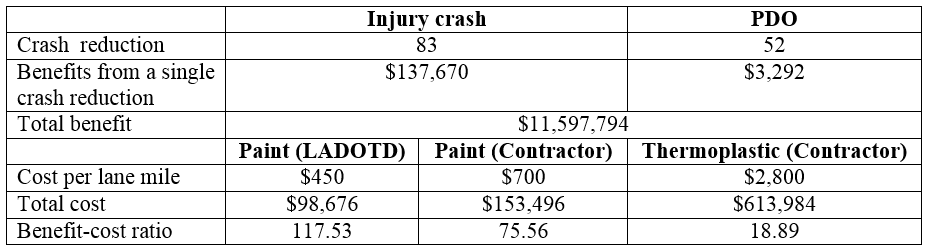
\includegraphics[width=10in, height= 2.5 in]{MD3.png}
                %\caption{The action of a quantum channel on its multiplicative domain.}
                %\label{fig:multDom}
              \end{center}
            \end{figure}
    \end{block}
    \vskip2ex




        \begin{block}{Significant Characteristics}

            \begin{figure}
              \begin{center}
                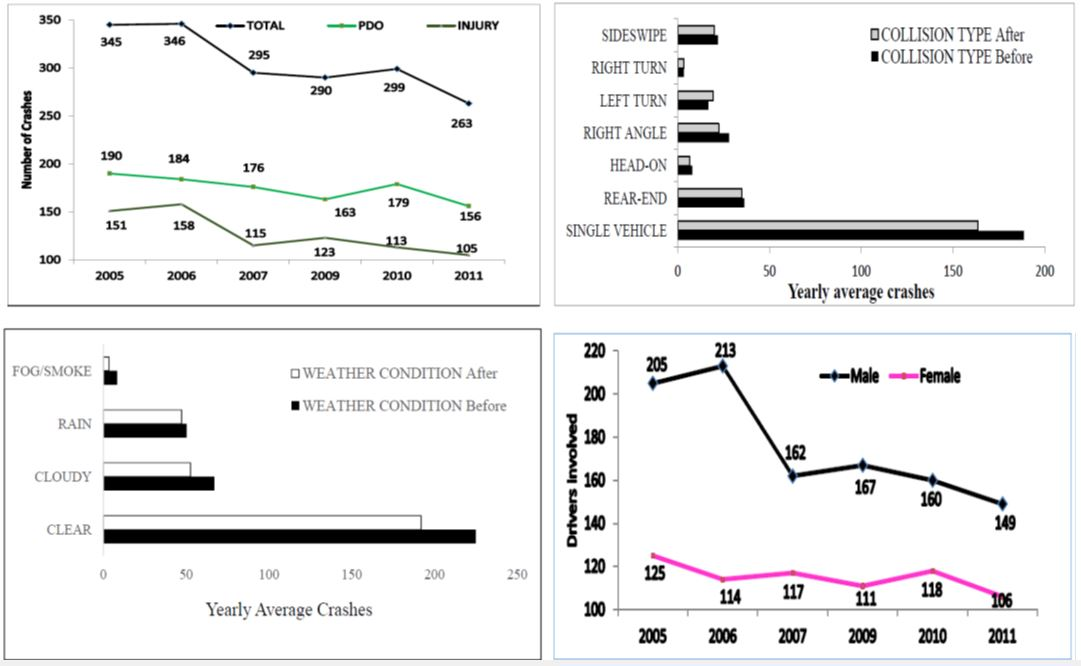
\includegraphics[width=10.5in, height=9in]{z11.jpg}
                \caption{Significant Characteristics}
                \label{fig:multDom}
              \end{center}
            \end{figure}
        \end{block}
    \vskip2ex



        \begin{block}{Crash Modification Factor (CMF)}
              {\rmfamily{
              The crash modification factor was estimated by the EB method with the crash data from three years before and after edge line implementation. Considering the crash overall decline between 2009 and 2011,the final estimated CMF for edge line implementation is 0.85 with a standard deviation 0.04, which means that the range of the estimation is between 0.73 and  0.96.}}



      \begin{center}
        \begin{tabular}{ccc}
          
\includegraphics[width=4in, height= 4in]{ulls.jpg} & \hspace{1.25in} & 
\includegraphics[width=4in, height=4in]{ltrc.jpg}
        \end{tabular}
      \end{center}
    \end{block}
  \end{column}
  \begin{column}{\sepwid}\end{column}			% empty spacer column
 \end{columns}
\end{frame}
\end{document}
